% Principios físicos. Leyes físicas, acoplamiento inductivo, modelo de las antenas, dependencia de k, L1, L2, como se mide en el estándar...
\chapter{Principio de funcionamiento}

Este capítulo describe los principios fundamentales de operación del sistema de RFID definido por el estándar ISO14443. Se abordarán primero los fenómenos físicos que posibilitan el enlace entre tranponder y lector para luego pasar a detallar como influyen en el diseño y caracterización de la interfaz de comunicación. Se desarrollará un modelo que contemple las características físicas más importantes del enlace y que será utilizado en los capítulos posteriores como base para el diseño y simulación de los circuitos electrónicos.

\section{Principios físicos de operación}

El sistema de RFID definido por el estándar utiliza el acoplamiento magnético existente entre dos inductores para transmitir tanto energía como información. Se trata de un fenómeno descripto por primera vez en el año 1831 por el físico \emph{Michael Faraday} en el que se observa como una corriente variable en el tiempo que atraviesa una bobina de alambre induce otra corriente en una espira cercana. El experimento puede esquematizarse con el arreglo de la figura \ref{fig:ExperimentoFaraday}, donde se observan dos espiras enfrentadas que comparten un eje común.

\begin{figure}
	\centering
	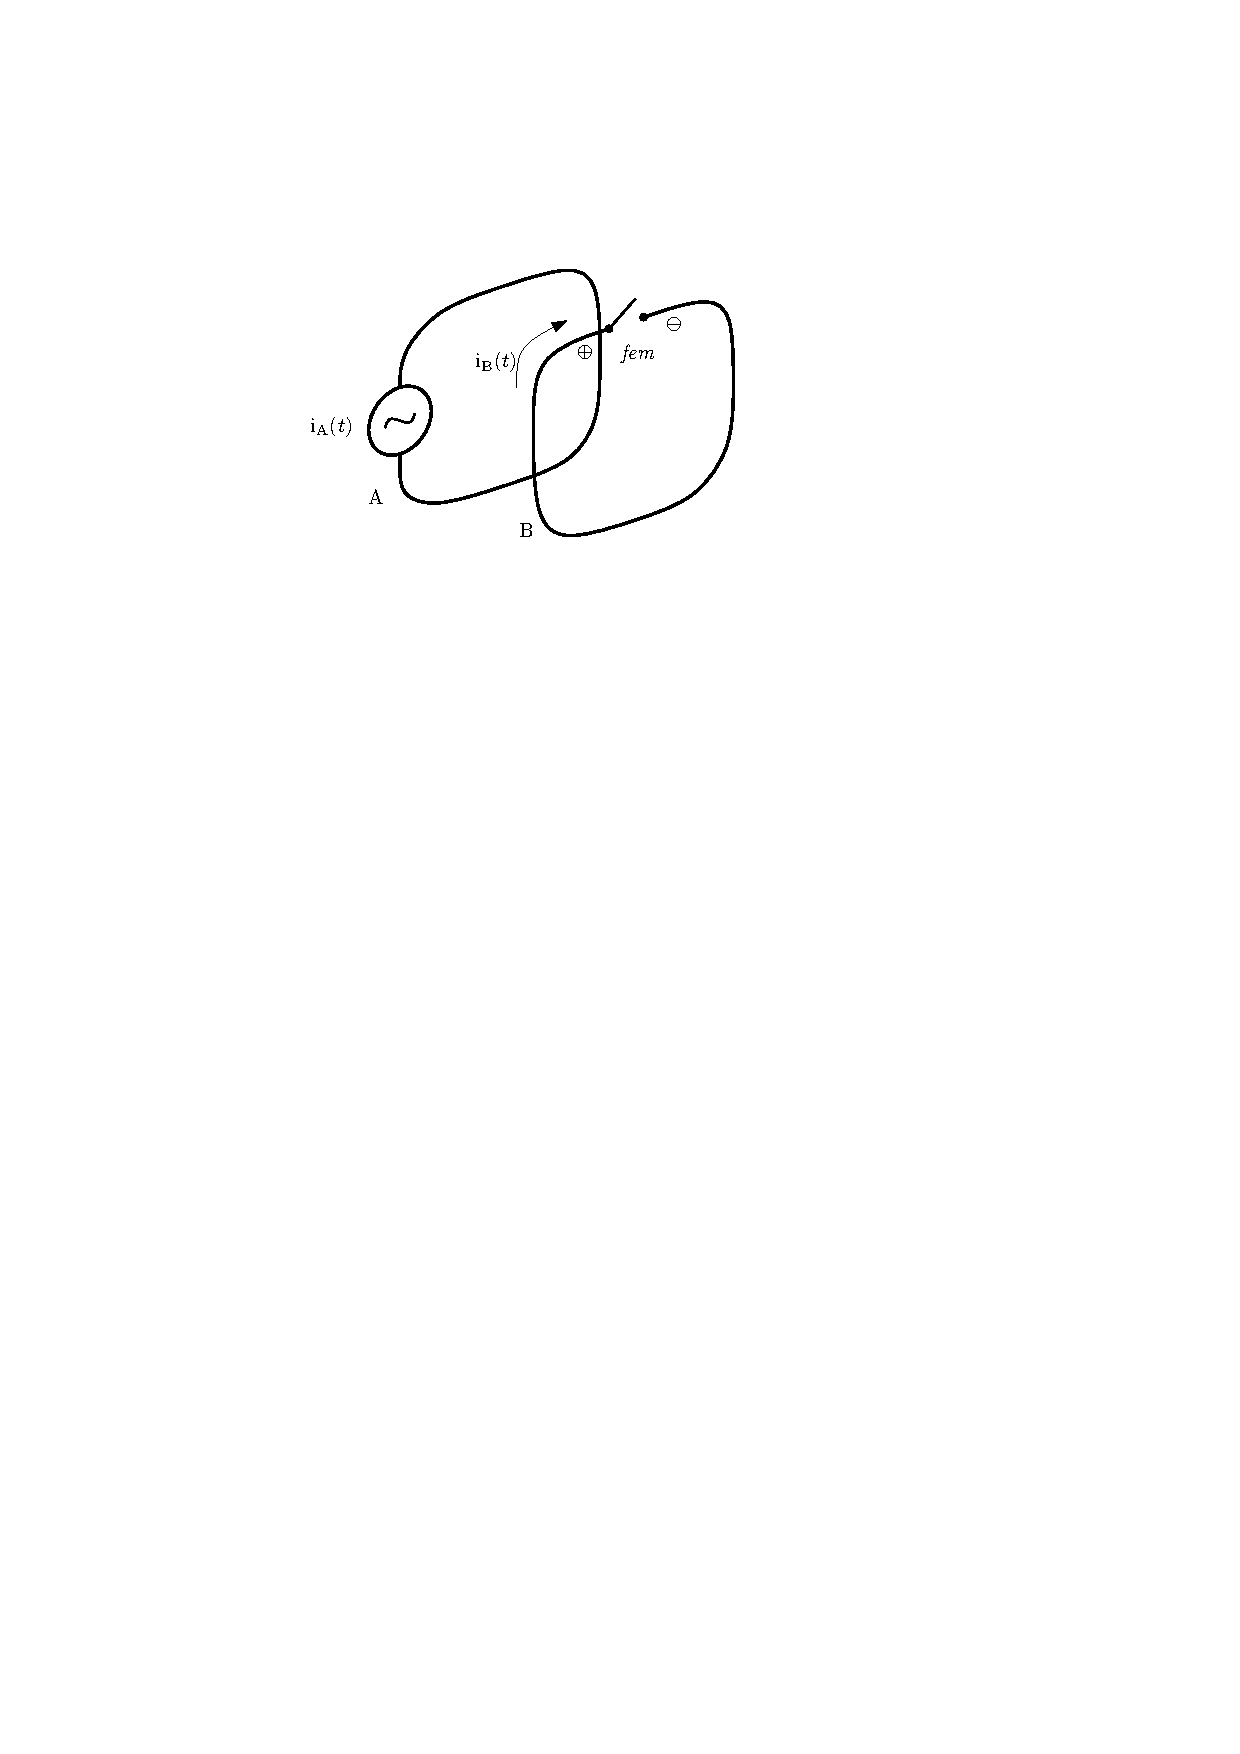
\includegraphics{ExperimentoFaraday}
	\caption{La corriente \(\mathrm{I}_\mathrm{A}\) induce una \emph{fuerza electromotriz} en el conductor B. Al cerrarse el circuito circula una corriente \(\mathrm{I}_\mathrm{B}\) que produce un campo magnético que interactúa con el generado por \(\mathrm{I}_\mathrm{A}\).}
	\label{fig:ExperimentoFaraday}
\end{figure}

La corriente que circula por el conductor A genera un campo magnético variable cuya expresión puede hallarse aplicando la \emph{ley de Biot-Savart}:

\begin{equation}
	\label{eq:EcBiot-Savart}
	\bar{B}(\bar{r}, t)=\frac{\mu_0}{4 \pi} \int_\mathrm{A} \frac{i_\mathrm{A}(t) \bar{\mathrm{d}l} \times \bar{r}}{|\bar{r}|^3}
\end{equation}

Donde \(\bar{\mathrm{d}l}\) es el vector diferencial de camino a lo largo de la espira A, \(\bar{r}\) es el vector que va desde la espira a cualquier punto del espacio y \(i(t)\) es la corriente que circula por la espira.

El campo magnético variable creado por la espira A induce una \emph{fuerza electromotriz} (\(fem\)) en el conductor B, cuya magnitud estará dada por la ley de \emph{Faraday-Lens}:

\begin{equation}
	\label{eq:EcFaradayLens}
	fem = - \frac{\mathrm{d}\Phi}{\mathrm{d}t} = - \frac{\mathrm{d}}{\mathrm{d}t} \int_\mathrm{B} \bar{B} \cdot \hat{n} \, \mathrm{d}S
\end{equation}

Al cerrarse el circuito en B, la fuerza electromotriz inducida hará circular una corriente \(\mathrm{I}_\mathrm{B}\) que a su vez creará un campo magnético opuesto al que le dio origen, interactuando de esta forma con la espira A. El flujo total de campo que atraviesa la superficie B está dado entonces por la suma de los campos producidos por \(i_A\) e \(i_B\).

En la ecuación \ref{eq:EcBiot-Savart} se observa que los campos magnéticos producidos dependen sólo de aspectos constructivos, como la forma y el tamaño de las espiras, y de la corriente que circula por ellas. Lo mismo sucede al calcular el flujo del campo a través de una superficie. Gracias a esto se define el parámetro L \emph{auto-inductancia}, o \emph{inductancia} a secas, de un conductor como el coeficiente que vincula el flujo del campo a través de la superficie encerrada por el conductor con la corriente que circula a través de él:
\[ L = \frac{\Phi}{i} \]

En el caso de la figura \ref{fig:ExperimentoFaraday}, donde el acoplamiento magnético se da entre dos conductores separados, también se define la \emph{inductancia mutua} M como el coeficiente que vincula el flujo de campo en la superficie encerrada por una de las espiras con la corriente que circula por la otra.
\[ M_{AB} = \frac{\Phi_A}{i_B} \]

Este coeficiente es simétrico, es decir \(M_{AB} = M_{BA} = M\).

Volviendo al cálculo de la \(fem\) en la espira B, puede aplicarse superposición para sumar los flujos debidos a \(i_A\) e \(i_B\). 
\[ fem = - \frac{\mathrm{d}}{\mathrm{d}t} \left( \Phi_{A} + \Phi_{B} \right)
\]

Utilizando las definiciones de auto-inductancia e inductancia mutua puede escribirse:

\[ fem = - \frac{\mathrm{d}}{\mathrm{d}t} \left( M \cdot i_A + L \cdot i_B \right) = -M \cdot \frac{\mathrm{d}i_A}{\mathrm{d}t} - L \cdot \frac{\mathrm{d}i_B}{\mathrm{d}t}
\]

Del experimento surge entonces que existe un acoplamiento magnético entre ambos conductores y que las variaciones de corriente en el conductor A se verán reflejadas en B y viceversa.


\todo{VER LO QUE ESCRIBI PARA TX Y RX.}Según la ecuación \ref{eq:EcFaradayLens}


